\begin{figure}[H]
\centering
\resizebox{0.94\textwidth}{!}{%
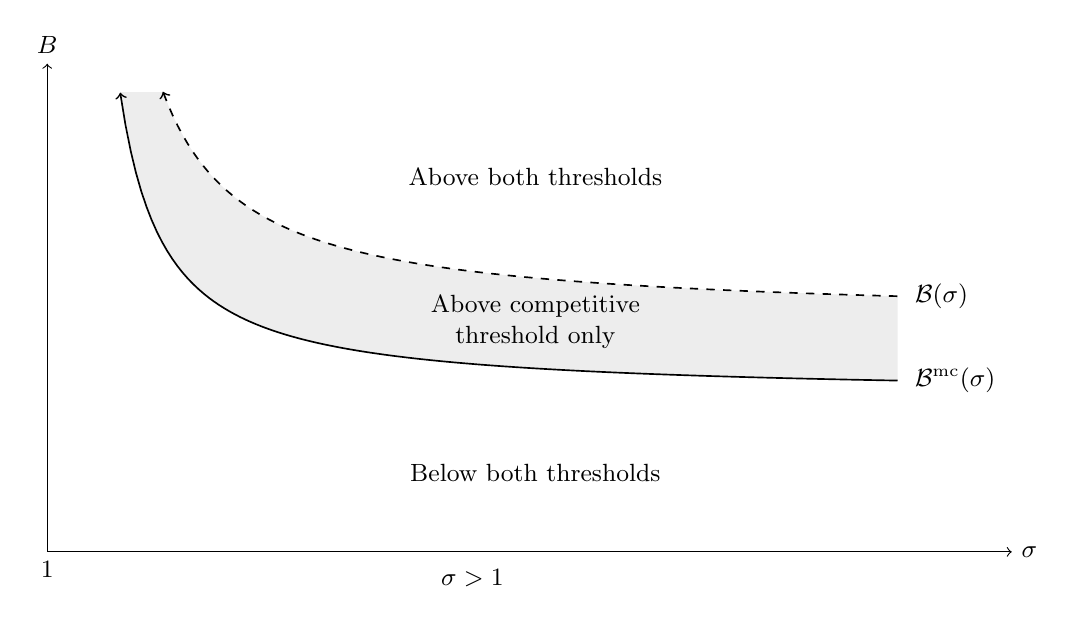
\begin{tikzpicture}[
 x=1.00cm,y=0.80cm,
 every node/.style={font=\small},
 region/.style={align=center,inner sep=3pt}
]
 \draw[->] (0,0) -- (12.25,0) node[right] {$\sigma$};
 \draw[->] (0,0) -- (0,7.75) node[above] {$B$};
 \node[below] at (0,0) {$1$};
 \node[below] at (5.40,-0.12) {$\sigma>1$};

 % Schematic coordinates only. The vertical ratio uses alpha=0.33,
 % the illustration in the preceding paragraph; no simulation is used.
 % Both branches diverge as sigma approaches one from above.
 \begin{scope}
  \clip (0,0) rectangle (10.80,7.30);
  \path[fill=black!7]
   plot[domain=0.80:10.80,samples=150] (\x,{3.7*exp(1/\x)})
   -- plot[domain=10.80:0.80,samples=150]
      (\x,{0.67*3.7*exp(1/\x)}) -- cycle;
 \end{scope}

 \draw[semithick,dashed,<-]
  plot[domain=1.47:10.80,samples=150] (\x,{3.7*exp(1/\x)});
 \draw[semithick,<-]
  plot[domain=0.927:10.80,samples=150] (\x,{0.67*3.7*exp(1/\x)});

 \node[anchor=west] at (10.90,4.06) {$\mathcal B(\sigma)$};
 \node[anchor=west] at (10.90,2.72) {$\mathcal B^{\mathrm{mc}}(\sigma)$};

 \node[region] at (6.20,5.95) {Above both thresholds};
 \node[region,text width=4.4cm] at (6.20,3.65)
  {Above competitive\\threshold only};
 \node[region] at (6.20,1.25) {Below both thresholds};
\end{tikzpicture}%
}
\caption{AI-efficiency thresholds under monopoly and competition.
For $\sigma>1$, marginal-cost pricing lowers the threshold to
$\mathcal B^{\mathrm{mc}}(\sigma)=(1-\alpha)\mathcal B(\sigma)$,
as established in Proposition~\ref{prop:rewrite-monopoly-threshold}.
The schematic compares pricing rules at a common efficiency $B$.
The equilibrium conditions instead compare $B_0$ with the competitive
threshold and $\overline B$ with the monopoly threshold; the diagram
does not rank equilibria from a common initial state.
Threshold equalities are not classified.}
\label{fig:rewrite-competitive-thresholds}
\end{figure}
